\documentclass[12pt,a4paper]{article}
\usepackage{hyperref}
\usepackage{graphicx}
\title{Laboratory 2: Unauthorized Access in Wireless Networks}
\author{Niclas Scheuing and Vasileios Dimitrakis}
\begin{document}
	\maketitle
	
	\section{Introduction}
	In this laboratory exercise, we learn about and experiment on the weakness in various wireless security mechanisms. More specifically, in the first chapter, we hack the MAC filtering, in the second one, we crack the WEP encryption and in the last part, we break the WPA2 Personal Passwords.
	
	\section{Materials and Methods}
	Throughout the lab exercise 2 we used different materials and methods, that are presented below:
	
	\begin{itemize}
		\item \emph{ifconfig}: Is used to configure the network interfaces.
		\item \emph{hostapd}: Is a user space deamon for Access Point and authentication servers.
		\item \emph{iwconfig}: Is used to configure the wireless network interfaces.
		\item \emph{iwlist}: Is used to display some additional information from a wireless network interface that is not displayed by iwconfig
		\item \emph{wireshark}: Is an open source packet analyser.
		\item \emph{macchanger}: Is a Linux command that changes the MAC address of a network interface.
		\item \emph{airodump-ng}: Is used for packet capturing of raw 802.11 frames and is particularly suitable for collecting WEP IVs (Initialization Vector) for the intent of using them with aircrack-ng.\cite{aircrack}
		\item \emph{aircrack-ng}: Is an 802.11 WEP and WPA-PSK keys cracking program that can recover keys once enough data packets have been captured. \cite{aircrack}
		\item \emph{ping}: Is a computer network administration software utility used to test the reachability of a host on an Internet Protocol (IP) network and to measure the round-trip time for messages sent from the originating host to a destination computer and back.
		\item \emph{wpa\_supplicant}: Is a cross-platform supplicant with support for WEP, WPA and WPA2.
		\item \emph{aireplay-ng}: Inject ARP-request packets into a wireless network to generate traffic.\cite{aircrack}
	\end{itemize}
	
	\section{Terminology}
	The machine serving as wireless node is denoted by \emph{User} and the machine used to attack the communication by \emph{Attacker}.
	The machine used as access point is called \emph{AP} in the following.
	
	
	\section{Experiments}
	In the following we will go through the experiments one by one and introduce the corresponding theory, setup and results.
	\subsection{Hacking MAC Filtering}
	\emph{MAC} filtering is a security technique to prevent unauthorized users from accessing a wireless network.
	All network devices have a unique 48bit \emph{MAC} address.
	The access-point grants or denies access to devices based on the \emph{MAC} address communicated by the device itself. This is why a device can spoof the \emph{MAC} address.
	For filtering black-lists and white-lists are used, granting access to devices contained in the white-list and denying access to those in the black-list.
	
	\subsubsection{Running the Experiment}
	\emph{AP} used a white-list containing the \emph{User's} \emph{MAC} address, but not the \emph{Attacker's} one.
	The \emph{AP} and the \emph{User} were transmitting data.
	The \emph{Attacker} was not able to connect to the \emph{AP}, because he was not on the white-list.
	
	To find the channel used for the communication and the \emph{AP's} \emph{MAC} address, the \emph{Attacker} used the \emph{iwlist} tool.
	The \emph{Attacker} was observing the communication running its Wifi adapter in \emph{monitor} mode and capturing the observed traffic with \emph{Wireshark}. In this way, he was able to extract the \emph{User's} \emph{MAC} address. See \autoref{mac:wireshark}
	
	Knowing this \emph{MAC} address, the \emph{Attacker} set his own \emph{MAC} address to the \emph{User's} address using the \emph{macchanger} tool. See \autoref{mac:changer}.
	The \emph{Attacker} \emph{User} were then able to connect to the \emph{AP}.
	
	\begin{figure}
		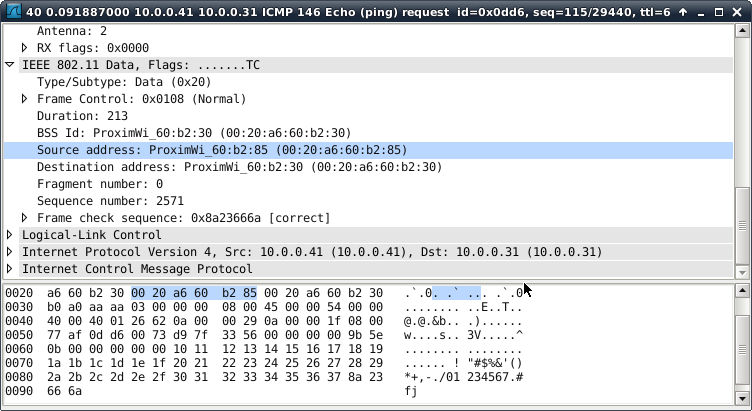
\includegraphics[width=\textwidth]{"images/other/im3.png}
		\caption{Finding the \emph{User's} \emph{MAC} address using \emph{Wireshark.}}
		\label{mac:wireshark}
	\end{figure}
	
	\begin{figure}
		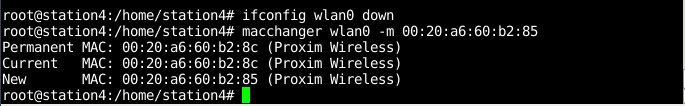
\includegraphics[width=\textwidth]{"images/other/im4_cut.png}
		\caption{Changing the \emph{Attacker's} \emph{MAC} address using \emph{macchanger.}}
		\label{mac:changer}
	\end{figure}
	\subsubsection{Analysis}
	\emph{MAC} filtering can easily be bypassed with some limitations. The \emph{Attacker} does not get his own \emph{MAC} address, but share it with the \emph{User}, which leads to undesired side effects, such as both receiving the same packages. Although, it is very easily implemented and it does not introduce additional overhead, which would reduce the networks throughput. Moreover, although it has this severe security flaw, nowadays it is used in wired networks, because it is harder for the \emph{Attacker} to sniff valid \emph{MAC} addresses. Furthermore, it can be used in small WLANs, where the users trust one another.
	
	When doing the measurements of our Cantenna, we used \emph{MAC} filtering with a white-list as a simple security mechanism to disallow other devices to simply connect to our access point. Only little computational and little data overhead was introduced and for this setting the amount of security was enough.1
	
	\subsection{Cracking WEP Encryption}
	WEP is security mechanism for wireless networks using a RC4 encryption with a 40bit \emph{secret} concatenated with a 24bit initialization vector. This key is usually represented as a string of 10 hexadecimal values. Besides the initialization vector, there is no additional randomness in the key used for the encryption, because the \emph{secret} remains the same over all transmissions. 24bit is short enough to be brute-forced.\cite{wep}
	
	\subsubsection{Running the Experiment}
	\emph{User1} and \emph{User2} were connected in ad-hoc mode using a WEP encryption.
	At first they used a different \emph{secret} each, and observed, they were not able to connect. Then they used the same \emph{secret} and could establish a connection.
	
	The \emph{Attacker} who did not set any key, could not connect.
	The \emph{Attacker} did observe the network using the monitor mode and wireshark.
	The packets sniffed using wireshark can be seen in \autoref{wep:wireshark}. It was a flood of ping messages, but encrypted with the WEP's RC4 encryption.
	
	The \emph{Attacker} then started the \emph{airodump-ng} to collect the traffic and \emph{aircrack-ng} tool to crack the key. See \autoref{wep:airodump}.
	It had to capture 38989 initialization vectors and based on that the tool had to try 236 keys to successfully guess the correct one. This took 7 seconds.
	The \emph{Attacker} could then join the network using the found key.
	
	This attack requires a few thousand captured packets. Depending on the network activity, this will take from a few seconds up to 10 minutes.
	
	Observing the traffic in our home network generated by a file server, a multimedia station and a notebook running, we got about 5000 packets per minute. So the attack would take a few minutes.
	
	In a office network with more traffic, this time would be significantly shorter.
	
	
	\begin{figure}
		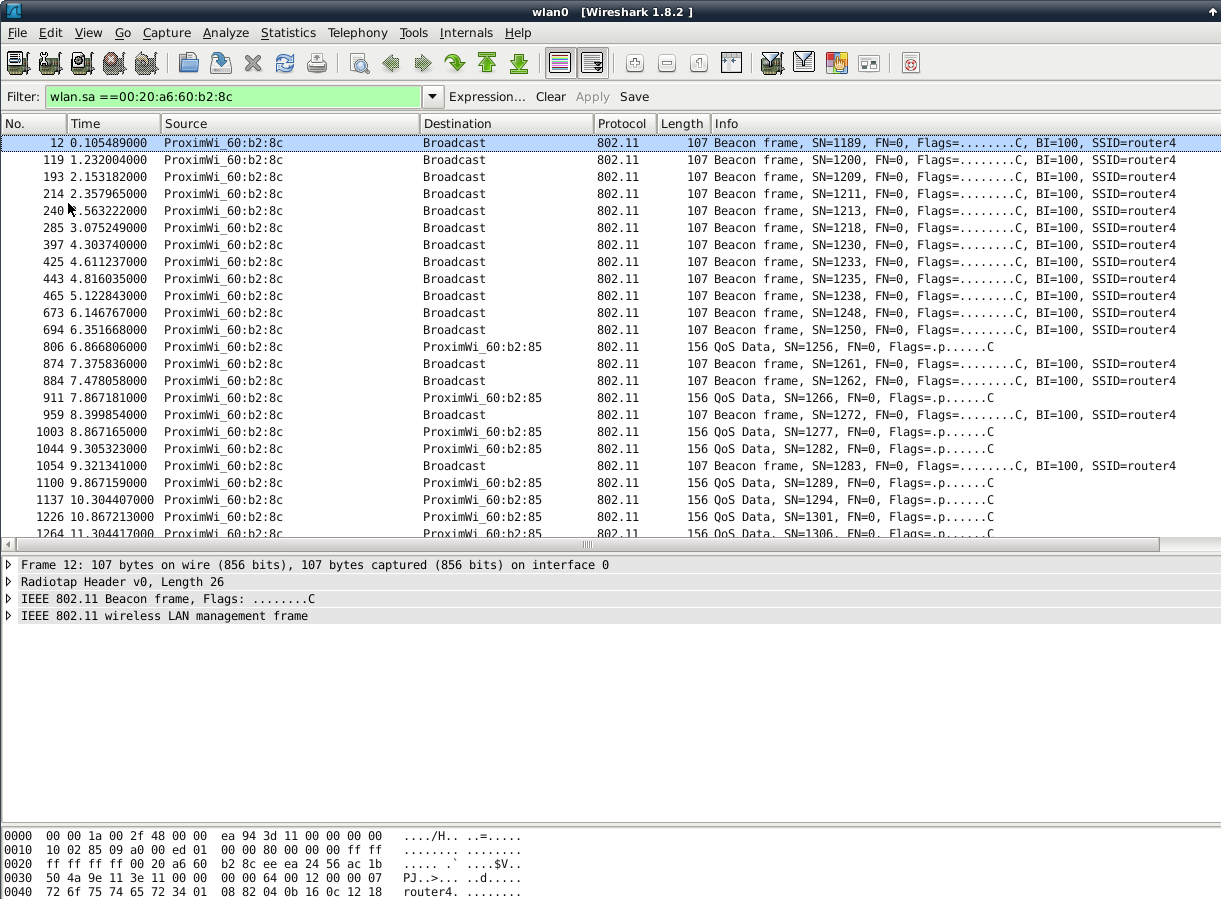
\includegraphics[width=\textwidth]{images/bill/pic1.png}
		\caption{Capturing the traffic using source \emph{MAC} address filtering.}
		\label{wep:wireshark}
	\end{figure}
	\begin{figure}
		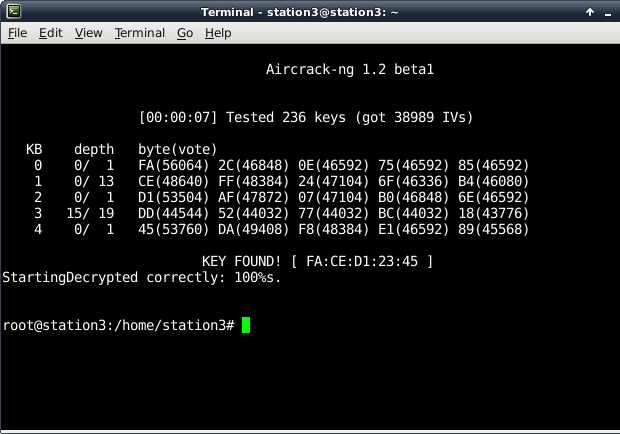
\includegraphics[width=\textwidth]{images/bill/pic3.png}
		\caption{Cracking the WEP key using \emph{aircrack-ng}}
		\label{wep:airodump}
	\end{figure}
	
	\subsection{Breaking WPA2 Personal Passwords}
	To deal with the weaknesses of WEP, WPA was introduced. WPA2 provides a mode using AES encryption with a 256bit key. It can be run in the \emph{personal mode} using pre-shared keys or the \emph{enterprise mode} using authentication protocols.
	
	To establish a session key, the WPA2 protocol performs a 4-way handshake between the access point and the client. During this a \emph{Message Integrity Check (MIC)} is computed and transmitted. The computation of the MIC uses the pre-shared \emph{Pairwise Master Key (PMK)}. An attacker can capture this handshake and break the MIC by brute-forcing the PMK.
	
	\subsubsection{Running the Experiment}
	\emph{AP} and \emph{User} are connected using a WPA2-PSK-AES setup in infrastructure mode. The key used was \emph{motorbike}, a word which is part of most dictionaries used for cracking passwords.
	
	The \emph{Attacker} was not able to connect without knowing the password, but could observes the encrypted traffic using wireshark.
	
	To get the \emph{MIC}, the \emph{Attacker} performed a de-authentication attack by sending de-authentication packets with \emph{aireplay-ng}.
	This caused the \emph{AP} and \emph{User} to reestablish the connection by performing the 4-way handshake.
	The handshake was captured by the \emph{Attacker} using \emph{airodump-ng}.
	\emph{aircrack-ng} cracked the MIC using the captured handshake and a dictionary.
	
	The machine the attack was performed could process \emph{3535.59 keys per second} or \emph{212135.4 keys per minute}. It took 10 seconds to find the password.
	
	This machine could perform \emph{305 Mkeys per day}.
	Since $\lg(305000000) \approx 28$, the a key with more than 28 bits could not be cracked within a day.
	
	This attack was possible, because the password was contained in the dictionary. Using a more random password would have prevented a simple dictionary attack.
	
	if password is long or not in dictionary, it is not possible for the attacker to retrieve the password.
	\begin{figure}
		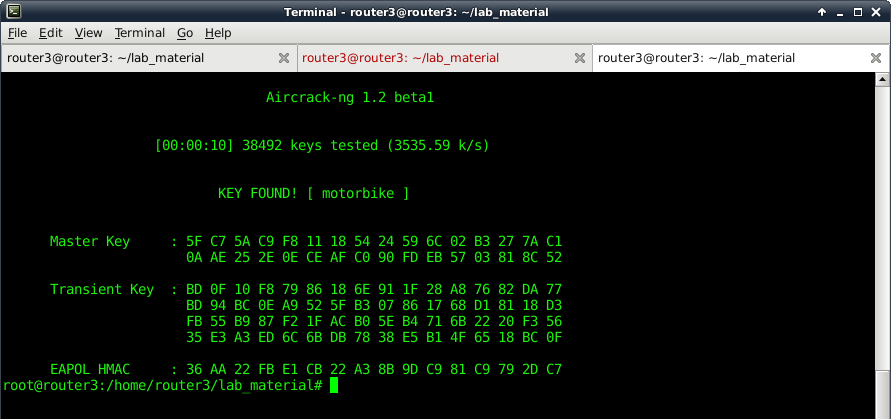
\includegraphics[width=\textwidth]{"images/nick/cracked_wpa2_cut.png}
		\caption{Cracked the WPA2 password with \emph{aircrack-ng}.}
		\label{wpa:crack}
	\end{figure}
	
	\section{Analysis}
	In this lab we demonstrated that some widely used security mechanisms as MAC-filtering, WEP and WPA2 are prone to rather simple attacks.
	\begin{itemize}
		\item \emph{MAC filtering:} As we mentioned in the introduction, this security technique is quite simple, but it can be overpassed easily enough. For this reason, nowadays it is not often used and the only cases that is implemented are in wired networks and small WLANs, where the packet sniffing is difficult and there is mutual trust between the users, respectively.
		
		\item \emph{WEP encryption:} This security method is also quite simple, but it offers weak protection and it is very easily exploited, due to specific inherent vulnerabilities of the protocol, such as small length of the IVs.
		
		\item \emph{WPA2 encryption:} WPA2 personal is the most secure technique of the other two ones. It uses block cipher for the encryption mode and this increases the process time. Although, WPA2 personal seems to be secure, it is susceptible to dictionary attacks, which can be avoided, if the user chooses a stronger password. 
		
		
	\end{itemize}
	
	
	\bibliographystyle{plain}
	\bibliography{bibliography}
\end{document}\grid
